%! suppress = FileNotFound
\documentclass[../main]{subfiles}

\begin{document}
\chapter[\tested{}-\dsl: a \dsl{} for creating programming exercises]{\tested{}-\dsl: a domain-specific language for creating programming exercises}\label{ch:tested-dsl}

Automated software testing is widely used in programming education to validate the correct behavior of submissions for programming exercises.
There are two dominant testing approaches: I/O-stream testing and unit testing.
I/O-stream testing is largely independent of the programming language, but its black-box nature makes it difficult to provide detailed feedback.
Unit testing, on the other hand, typically requires a separate test suite for each target programming language.

This chapter introduces TESTed-DSL as a domain-specific language (DSL) designed to simplify authoring language-agnostic test suites for programming exercises with automated assessment support.
Test suites written using TESTed-DSL
\begin{enumerate*}[label=\emph{\roman*})]
    \item share the same declarative structure and testing functionality across programming languages,
    \item bridge the gap between I/O-stream testing and unit testing, and
    \item allow for expressing test code in a language-agnostic way.
\end{enumerate*}
The educational software testing framework TESTed allows for automated assessment using language-agnostic test suites expressed in TESTed-DSL, as demonstrated in a case study.
Additionally, TESTed now includes a template engine based on TESTed-DSL for authoring task descriptions that include language-agnostic specifications of data types, literal values, identifiers, and code fragments.

\section{Background and motivation}\label{sec:dsl-background-and-motivation}

\subsection{Educational software testing}\label{subsec:dsl-educational-software-testing}

Software testing is the validation and verification of a system derived from source code~\autocite{ammannIntroductionSoftwareTesting2016}.
Two complementary approaches prevail: dynamic testing executes the source code with a given suite of test cases, whereas static testing analyzes the source code without executing it~\autocite{romliAutomaticProgrammingAssessment2010}.
Both approaches might be done via manual or automated processes, based on a specification~\autocite{pieterseAutomatedAssessmentProgramming2013}.
In modern software development, automated testing has become a standard practice for continuous integration and continuous development of living codebases, where both the codebase and the system requirements might evolve over time~\autocite{wintersSoftwareEngineeringGoogle2020}.
The minimum requirement that is tested is correctness, which is the essential purpose of software testing~\autocite{panSoftwareTesting1999}.
The desired or correct behaviors are specified as the functional requirements of the program and say how a program must behave~\autocite{bassSoftwareArchitecturePractice2021}.
Automated testing for correctness needs some kind of oracle to tell if the functional requirements are satisfied.
Other software quality factors (the non-functional requirements) that may be tested are its functionality (reliability, usability, integrity), engineering (efficiency, testability, documentation, structure) and adaptability (flexibility, reusability, maintainability)~\autocite{hetzelCompleteGuideSoftware1988}.

Educational software testing is the application of automated software testing to source code students submit for programming exercises~\autocite{staubitzRepositoryOpenAutogradable2017,paivaAutomatedAssessmentComputer2022,souzaSystematicLiteratureReview2016,keuningSystematicLiteratureReview2018}.
For brevity, the source code under test will be called submissions throughout this paper.
What makes educational software testing unique is that each programming exercise has a fixed specification, against which multiple submissions must be validated and verified~\autocite{wilcoxTestingStrategiesAutomated2016}.
Submissions are usually small to moderate in size, with all source code contained in a single file in most cases.
The main purpose of educational software testing is automated assessment of submissions~\autocite{berssanetteActiveLearningContext2021}, which may come as feedback and/or as a grade~\autocite{caizaProgrammingAssignmentsAutomatic2013}.
Assessments can be provided instantly upon each submission while students work on their solution.
Such a continuous assessment provides ``feed back'' on how students performed and ``feed forward'' on what to do next before making a new submission for the same assignment~\autocite{cheangAutomatedGradingProgramming2003,higginsCourseMarkerCBASystem2003,luckSecureOnlineSubmission1999}.
Assessments can also happen after a submission deadline has passed, and provide students ``feed back'' on their overall performance~\autocite{hattiePowerFeedback2007,timmisRethinkingAssessmentDigital2016}.

\subsection{Programming exercises}\label{subsec:dsl-programming-exercises}

Efforts to standardize the representation of programming exercises have been numerous, encompassing various strategies, such as combining the metadata, assets and task description into one formally structured document~\autocite{mishraProgrammingExerciseMarkup2023,paivaAnotherProgrammingExercises2020,queirosPexilProgrammingExercises2011,swachaSIPEDomainspecificLanguage2018}, a predefined directory structure~\autocite{verhoeffProgrammingTaskPackages2008}, or a combination thereof~\autocite{edwardsDevelopingCommonFormat2008a,strickrothProFormAXMLbasedExchange2015}.
The objective of these initiatives is laudable: increasing the \textsc{fair}ness of programming exercises as digital educational resources that are findable, accessible, interoperable and reusable~\autocite{wilkinsonFAIRGuidingPrinciples2016}.
Without exception, all of them support (automated) assessment as a feature, showing its importance for programming exercises.
However, due to their generic nature, these exercise standards only provide support for assessment metadata and assets, and leave the actual representation of test suites, software testing frameworks, and dependencies on runtime environments open for implementation.
But to make programming exercises truly interoperable, test suites and testing frameworks are no implementation detail.
As a result, any promise of plug-and-play programming exercises that can be freely exchanged between learning platforms has not yet been resolved~\autocite{ala-mutkaSurveyAutomatedAssessment2005,ihantolaReviewRecentSystems2010,messerAutomatedGradingFeedback2024,paivaAutomatedAssessmentComputer2022}.

In this chapter, we do not focus on the overall representation of programming exercises as such, but rather on the specific aspects of task descriptions and test suites, which are key for automated assessment.
We explore how to design programming exercises that can be assessed automatically across different programming languages.
This capability is essential for creating exercises that accept submissions in various languages and allow for dynamic testing using a single test suite~\autocite{staubitzPracticalProgrammingExercises2015}.
For that purpose, test suites capturing the requirements of programming exercises must ideally be specified in a language-agnostic way.
We focus in the first place on validating the correctness of submissions as a way of formative feedback, and not per se on grading submissions as a way of summative feedback.

Designing programming exercises that apply across programming languages is relevant in educational practice~\autocite{murphyAnalysisIntroductoryProgramming2017}.
Exercises whose primary focus is problem-solving, data structures or algorithms are by nature only loosely bound to a particular programming language, so teachers may want to leave the choice of language to individual students.
This is especially useful in courses taken by mixed populations of students trained in different programming languages or where choice of the most appropriate language is an explicit challenge in the problem-solving process.
But even programming courses that teach a particular programming language might benefit from exercise repositories built around the \textsc{fair}-principles, where exercises restricted to a single programming language are simply less reusable.

\subsection{I/O-stream testing}\label{subsec:dsl-i/o-stream-testing}

The need for programming exercises supporting automated assessment across programming languages is also reflected by the fact that the most often used architecture for test automation in educational practice is based on standard I/O streams~\autocite{douceAutomaticTestbasedAssessment2005,ullahEffectAutomaticAssessment2018,wasikSurveyOnlineJudge2018}.
The only language-specific step with such a data-driven approach is the optional compilation and then execution of submissions, which read from the standard input stream (stdin) and write to the standard output streams (stdout and stderr).
This approach is broadly applicable, as almost all programming languages support standard I/O-streams.

Testing itself treats submissions as black boxes by streaming input data via stdin, capturing output data via stdout and stderr, and running standalone test oracles to validate the correctness of the output data generated by the submission (\vref{fig:io-testing}).
Teachers can describe the task specification of I/O-stream-based exercises to students, independent of any programming language.
Such a task description only specifies the formatting of input and output data, and prescribes how input data must be transformed into output data.

\begin{figure}
    \centering
    \includestandalone{io-testing}
    \caption{Architecture of a test execution engine based on standard I/O-streams. The entry point of the program execution (often the main function) and the standard I/O-streams are the only interface for reaching into and revealing internal behavior of the submission. Assessing the submission for a single test case comes down to running the executable (thick bordered boxes) with \textcolor{input-green}{input data} streamed to standard input (stdin), capturing \textcolor{output-blue}{output data} from its standard output and error streams (stdout and stderr), and running standalone oracles to validate whether the output data generated by the submission satisfies the requirements from the task description.\label{fig:io-testing}}
\end{figure}

The black-box and weakly typed nature of I/O-stream testing comes with serious pedagogical downsides.
The I/O-streams are the only interfaces for reaching into and revealing internal behavior of the submission.
While other data flows and user interactions are possible in software applications~\autocite{khorramTestingFrameworkExecutable2022}, they cannot be used here.
As students can only use the execution entry point (often the main function), only the behavior of the submission as a whole can be tested.
Individual steps (e.g.\ functions or classes) are not reachable.
Feedback can thus only be provided at a holistic level.

Although standard I/O-streams may in theory consume and produce binary data, programming exercises commonly use text-formatted input and output data.
Implementing the interface thus involves parsing a weakly typed external string representation of input data into a strongly typed internal representation, and converting a strongly typed internal representation of output data into a properly formatted external string representation that is used for validation.
As a result, test oracles have to process weakly typed output data as well.

\subsection{Unit testing}\label{subsec:dsl-unit-testing}

Unit testing largely resolves these issues.
Unit testing frameworks have become the norm in software development practice~\autocite{runesonSurveyUnitTesting2006}, and have also found their way into educational practice~\autocite{bettiniEnvironmentSelfassessingJava2004,ellsworthQuiverSystem2004}.
Such frameworks run test cases as scripts that access internal interfaces from specific sections (units) of the submission and rely on oracles to validate that the units behave as intended.
A unit could still be the entire submission (e.g.\ by calling the main function), but more commonly it is an individual function (in procedural or functional programming) or an individual class that is accessed through its public properties and methods (in object-oriented programming).
By first writing tests for the smallest testable units, and then compound behaviors between those, one can gradually build up comprehensive tests for more complex programming exercises~\autocite{panSoftwareTesting1999}.
In addition, oracles can process strongly typed values returned by calling functions or methods or by accessing properties, allowing for more versatile correctness testing (e.g.\ testing real-valued numbers are correct up to an expected accuracy).

Traditional unit testing frameworks compile the submission along with the test script and oracles into a single executable called a test harness (\vref{fig:unit-testing}).
As a consequence, they often require the test script and oracles to be written in the same programming language as the submission.
This restriction is rarely problematic in software development practice \emph{sensu latu}, but hampers accepting submissions in multiple programming languages in an educational context, unless separate test suites are provided for each target language.
This not only duplicates work, but unit testing frameworks for different languages also dictate how test suites are written~\autocite{agrawalSurveyGradingFormat2022,nayakAutomatedAssessmentTools2022}, which differs from framework to framework.

\begin{figure}
    \centering
    \includestandalone{unit-testing}
    \caption{Architecture of a unit test execution engine. Assessing a submission for a single test case comes down to compiling the submission along with the test code (including test script and oracles) into an executable test harness (thick-bordered box). The test script consists of a set of statements and expressions. The harness executes the test script, whose statements and expressions may access public interfaces of a narrow section of the submitted code (unit), captures \textcolor{output-blue}{outputs} (return values, exceptions) when executing statements and expressions in the script, and runs oracles to validate these outputs.\label{fig:unit-testing}}
\end{figure}

\subsection{TESTed 1.0}\label{subsec:tested-1.0}

We introduced TESTed~\autocite{strijbolTESTedEducationalTesting2023} (see also \vref{ch:tested1}) as an open-source educational software testing framework that accepts submissions in multiple programming languages and performs both I/O-stream testing and unit testing, based on a single language-agnostic test suite.
Currently, TESTed supports evaluating submissions in Bash, C, C\#, Haskell, Java, JavaScript, Kotlin, and Python.
Its abstract programming language engine transforms between language-agnostic and language-specific representations of strongly typed values, expressions, and statements.
This allows TESTed to generate language-specific test harnesses by converting language-agnostic test scripts on the fly into the programming language of a submission (\vref{fig:tested-testing}).
Executing a language-specific test harness yields strongly typed objects in a language-specific representation.
The language-specific test harness then converts these objects back into abstract form before exporting them to a language-agnostic test harness for validation by oracles that run independent of the language-specific test harness.

\begin{figure}
    \centering
    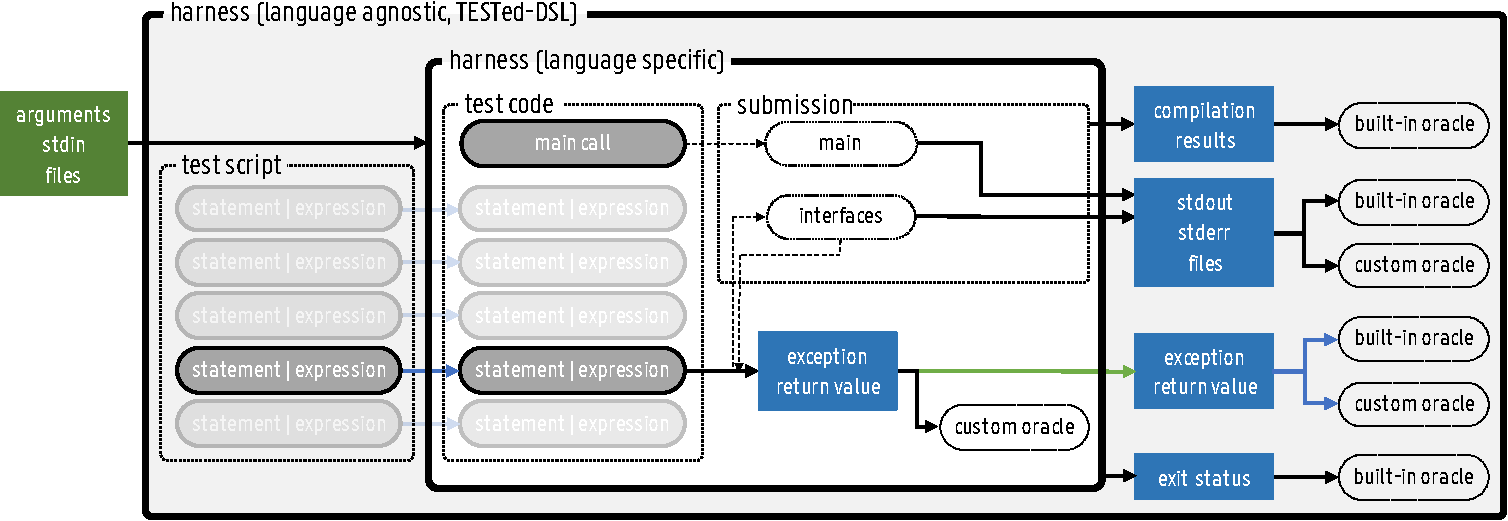
\includegraphics[width=\textwidth]{tested-testing}
    \caption{
        Architecture of the test execution engine of TESTed.
        Since TESTed supports both I/O-stream testing and unit testing, its architecture is a combination of Figures~\ref{fig:io-testing}~and~\ref{fig:unit-testing}.
        TESTed achieves this by running a language-specific harness (white box) within the language-agnostic test harness (grey box).
        Assessing a submission for a single test case again comes down to compiling the submission along with test code into an executable test harness.
        The \textcolor{input-green}{input data} are passed to the executable, and the test script consists of a set of statements and expressions.
        However, the strongly typed values, expressions and statements in the test script may now be in a language-agnostic representation.
        Before compilation, the test script is transformed (blue arrows) into language-specific test code.
        While the main call interacts with the main function of the submission, other tests access public interfaces of the submission (a single statement/expression is illustrated here).
        If a language-specific oracle is used, it is included in the language-specific harness.
        Otherwise, the strongly-typed \textcolor{output-blue}{outputs}, together with the \textcolor{output-blue}{outputs} from the main function, are processed in the language-agnostic harness.
        To make this possible, strongly-typed \textcolor{output-blue}{outputs} are transformed from a language-specific representation into a language-agnostic representation (green arrow).
        Finally, oracles in the language-agnostic harness evaluate the outputs.
        To make this possible, strongly typed values are converted in to the language-specific representation of the oracle (blue arrow).\label{fig:tested-testing}}
\end{figure}

\subsection{Organization of this chapter}\label{subsec:dsl-organization}

This chapter introduces TESTed-DSL as a domain-specific language (DSL) to simplify authoring test suites for language-agnostic programming exercises with support for automated assessment (\vref{sec:tested-dsl}).
We investigate its versatility, expressiveness, and general features by extending TESTed with support for the DSL\@.
This yields an open-source implementation of the DSL itself.
It also replaces the verbose and ad-hoc JSON specification of test suites from TESTed version 1.0, which closely followed the internal representation of test suites.
Statements and expressions of the abstract programming language, for example, were expressed in JSON as hierarchical structures that resemble abstract syntax trees (AST).

We then apply TESTed-DSL to task descriptions (\vref{subsec:dsl-language-agnostic-task-descriptions}), which allows authors of programming exercises to create task descriptions with language-specific programming interfaces (data types, literal values, identifiers, and code fragments) expressed in a language-agnostic way.
A template engine then transforms the language-agnostic interface bindings into specific representations for any target programming language supported by TESTed, while preserving other formatting of task descriptions.

This is followed by a set of examples illustrating the use of TESTed-DSL (\vref{sec:dsl-illustrative-examples}).
We then elaborate on a case study of using TESTed-DSL in educational practice (\vref{subsec:dsl-expressiveness-and-ergonomics}) and analyze the performance of running the testing framework from the DSL (\vref{subsec:dsl-performance}).
The results and impact of our contributions are discussed at length (\vref{sec:dsl-results-and-contributions}).
We conclude that extending TESTed with a DSL for specifying test suites and task descriptions provides an expressive and ergonomic solution.
It allows for authoring a diverse set of language-agnostic programming exercises that support automated assessment in educational practice.
We close by drawing the roadmap for some ongoing and future work (\vref{sec:dsl-conclusion-and-future-work}).

\section{\tested{}-\dsl{}}\label{sec:tested-dsl}

TESTed-DSL was conceived as a domain-specific language (DSL) for language-agnostic test suites of programming exercises that support automated assessment.
Such a test suite generally consists of two parts: individual tests (including test data) and a structured grouping of tests into units.
In this section, we first introduce the structure of the DSL, followed by the abstract programming language that is used to represent test data, expressions, and statements.

\subsection{Test suite structure}\label{subsec:dsl-test-suite-structure}

\begin{listing}
    \begin{minted}{yaml}
- unit: "Greet function"
  cases:
    - expression: "greet('World')"
      return: "Hello, World!"
    \end{minted}
    \caption[]{
        ``Hello, World!'' example of the specification of a test suite in TESTed-DSL.
        The test suite has a single test case that calls the function \texttt{greet} with string argument \texttt{"World"}.
        The function is expected to return the string \texttt{"Hello, World!"}.
    }
    \label{lst:yaml-basic-example}
\end{listing}

TESTed-DSL uses YAML~\autocite{ben-kikiYAMLAinMarkup2021} as a markup language for describing test suites that are preferably specified in a language-agnostic way.
The structure of test suites is formally specified in a JSON Schema\footnote{\url{https://github.com/dodona-edu/universal-judge/blob/master/tested/dsl/schema.json}}.
Note that this schema can be plugged into text editors or integrated development environments (IDE) for syntax highlighting, autocompletion, and validation.
\Vref{lst:yaml-basic-example} shows a minimal example of a test suite.
More elaborate examples are discussed in \vref{sec:dsl-illustrative-examples}.
% TODO: use dodona terms or reverse?
The test suites have a hierarchical structure: a test suite may have multiple \textbf{units}.
Each unit is tested by multiple \textbf{test cases}.
A test case consists of \textbf{setup} code, an optional \textbf{main call}, a \textbf{script}, and \textbf{teardown} code.
The DSL has an identical structure to JSON test suites (\vref{subsec:structure-of-a-test-suite}).
The minimal example has a single unit with a single test case, and no setup, main call, nor teardown.
The main call and the script together comprise the \textbf{tests} for the test case (Figure~\ref{fig:tested-testing}).

The input data for the main call is made available as \textbf{files}, passed as \textbf{arguments}, streamed through standard input (\textbf{stdin}), or any combination thereof.
The input data for the script are the \textbf{statements} and \textbf{expressions} it consists of.
The minimal example has a single script with a single test expression.
However, in TESTed-DSL, there is no separation between these types of tests: all tests (the main call and the script) are given as individual tests of a test case.
The type of the test is automatically derived from the available input.
If stdin or arguments are present, the test is considered to be a main call and will be executed as such.

When TESTed runs a test, it catches any \textbf{runtime exception} and output sent through the standard output streams (\textbf{stdout} and \textbf{stderr}).
It also catches the \textbf{return value} when expressions are evaluated (as is done in the minimal example) and the \textbf{exit status} when the process running the language-specific test harness terminates.

Test suites can specify a value for each possible input and an expected value for each possible output of a test.
Most inputs and outputs of tests are weakly typed: arguments, I/O-streams, (text) files, and messages of runtime exceptions are always strings, and the exit status is always an integer.
Return values, on the other hand, are strongly typed.

The validation of the actual values against the expected values happens with oracles.
By default, the built-in oracles of TESTed are used with default expected values.
For example, an exit code must be 0, and there must not be any output on stderr.
To avoid unnecessary feedback, correct tests against a default value are not reported.
For example, if the exit code of the submission is not zero, this will be reported as a failure.
However, it is distracting to show a successful zero exit code for all test cases (e.g.\ even those that test function calls).
For that reason, the exit code test is typically hidden.
In the minimal example, the exit code would be checked, but not reported unless it was non-zero.

For all outputs, the built-in oracles perform equality testing: the actual value must match the expected value.
However, the built-in oracles feature adjustable parameters that offer a degree of flexibility in this equality testing.
Examples include case-insensitive comparisons for strings and a tolerance for slight inaccuracies in real number comparisons.
Importantly, these parameter settings adhere to an inheritance mechanism across the test suite hierarchy.
Setting a parameter at a certain node within the suite takes precedence over any similar setting at a higher level and extends to all subordinate nodes.

Custom oracles can also overrule built-in oracles for standard output streams (stdout and stderr) and return values.
Custom oracles are called with the expected and actual values, in addition to some metadata about the test.
These allow for custom validations beyond equality testing.
They can also be useful for non-deterministic results, e.g.\ results that depend on the current date.

\subsection{Abstract programming language}\label{subsec:dsl-abstract-programming-language}

TESTed-DSL adopts a subset of the Python programming language as the language-agnostic representation of expressions, statements, and strongly typed values.
The subset is deliberately chosen to suit the specific needs of language-agnostic test suites, and therefore does not encompass all Python features.

An expression in the abstract programming language may consist of literals, identifiers, function calls, constructors, method calls, and property access.
Functions, constructors, and methods take expressions as positional arguments or as named arguments.
A statement is either an assignment or an expression.
Unlike other programming languages, Python has no way to differentiate constructors from function calls.
Because that difference is important to make when transforming language-agnostic expressions into the specific syntax of some programming languages (e.g.\ using the \texttt{new} keyword), TESTed-DSL follows the convention that constructors call a function whose name begins with a capital.
Another convention is that variables that are all caps are considered global variables.
Otherwise, TESTed-DSL follows Python conventions where possible.

A strongly typed value is obtained when TESTed evaluates a test expression.
These return values can be denoted as native YAML scalars (\texttt{null}, \texttt{booleans}, \texttt{integers}, \texttt{real numbers}, and \texttt{strings}), \texttt{sequences}, \texttt{sets} (using the \texttt{!!set} tag), and \texttt{mappings}.
By default, TESTed-DSL resolves these YAML objects as basic types of TESTed.
Casting to advanced types of TESTed is possible by using explicit YAML data types (\texttt{!type} tag).
As such, an expected return value \texttt{42} with TESTed data type \texttt{int64} can be expressed as \texttt{!int64 42}.

YAML strings are interpreted as literal strings by default, but are interpreted as expressions in the abstract programming language when the \texttt{!expression} tag is used.
As a result, \mintinline{yaml}{!set [1, 2, 3]} can also be denoted as \mintinline{yaml}{!expression "set([1, 2, 3])"}.

\subsection{Language-specific test suites}\label{subsec:dsl-language-specific-test-suites}

As the abstract representation of TESTed-DSL is independent of any programming language, not every feature and data type of every programming language is supported.
Examples include object equality checking (in object-oriented languages) or pointers (in C).
To accommodate this, TESTed-DSL also supports language-specific representations.
The language-specific representations are copied verbatim into the language-specific test harness and bypass the language-agnostic harness.
This means that all language features of the programming languages can be used.

In addition to language-specific statements and expressions, TESTed also allows writing custom oracles for return values whose expected data type is not supported by the abstract representation of TESTed.
Because such oracles run inside the language-specific harness, they also bypass the need for transforming return values, as is the case for traditional language-specific unit testing frameworks.

However, these language-specific features have to be used sparingly, as they restrict testing to programming languages for which language-specific representations and custom oracles are specified.
\Vref{lst:javascript-test-suite} (in \vref{subsec:dsl-declarative-structure}) contains an example of a test suite that uses language-specific representations.

\subsection{Language-agnostic task descriptions}\label{subsec:dsl-language-agnostic-task-descriptions}

For automated assessment to work, task descriptions of programming exercises have to specify what the submissions must implement (the interface) and how submissions must behave (interactions with the interface).
The expected behavior prescribes what type of input data is passed when interfaces are accessed, what type of output data they must return and how they need to transform input data into output data.
When references to and interactions with these interfaces have specific bindings to programming languages, they result in language-specific task descriptions.
For example, if a submission must implement a function that filters a list, the naming convention of the function and the values passed to this function (a list) will look different depending on the programming language.

The same rationale for having a single, language-agnostic test suite also applies to task descriptions.
A similar approach to avoid the need to author language-specific task descriptions for each target programming language of an exercise can be followed.
There are some differences though.
First of all, language-specific interface references and interactions in task descriptions are usually embedded in natural language content formatted with some plaintext markup language (e.g.\ Markdown, HTML or reStructuredText).
We therefore extended TESTed with an engine that supports authoring task descriptions as Jinja2 templates\autocite{ronacherJinja} with language-agnostic interface bindings embedded as \mintinline{jinja}{{{binding}}} placeholders in plain-text documents.
The engine then automatically transforms each placeholder into a specific representation for any target programming language supported by TESTed, while preserving surrounding formatting of task descriptions.

For each type of interface with language-specific bindings, the engine provides a corresponding Python variable or function that identifies the interface.
Interface functions take a language-agnostic representation (a string) of the interaction as their first argument and return its corresponding language-specific representation (also a string) that replaces the placeholder.

Interface interactions in task description templates are natural counterparts of their representations in TESTed-DSL test suites: \textbf{statements}, \textbf{expressions}, and \textbf{literal values}.
However, in task description templates, the engine makes no difference between statements, expressions, and literal values.
All are represented as a statement.
For example, an expected return value of a function or method call is a statement.
To reference a named function, the snake case version of its identifier is passed to the function identifying the interface in TESTed-DSL's abstract programming language: variables (\texttt{variable}), functions (\texttt{function}), classes (\texttt{class}), methods (\texttt{method}), properties (\texttt{property}) and parameters (\texttt{parameter}).
The engine formats these according to the naming conventions for the target programming language.
For example, \mintinline{python}{function('the\_function')} will result in the string \texttt{TheFunction} in C\#.

In addition, the engine also exposes a \texttt{datatype} function, which can be passed the name of a basic or advanced data type.
For example, \mintinline{python}{datatype('integer')} denotes the basic type \texttt{integer}.
This function returns an object, that when converted to a string by the engine, results in the formal name in the target programming language.
The object also supports two properties: \texttt{singular} and \texttt{plural}.
These methods return the informal name for the type (in singular or plural form respectively) in the target programming language.

The engine also exposes some additional environment variables: the target programming language (\texttt{language}), the target natural language (\texttt{natural\_language}) and the namespace (\texttt{namespace}) that is specified for some languages.
These environment variables are particularly useful in combination with Jinja2 control structures, for example, to add language-specific sections to task descriptions.

Task description templates can also reuse the language-agnostic specifications of TESTed-DSL test suites for code fragments that illustrate the expected behavior of interfaces with example interactions corresponding to test cases.
The template engine renders these fragments in the style of Python doctests: language-specific statements with language-specific string representations of expected outputs.
In task description mode, the engine ignores features of test suite specifications that steer the testing process.
For example, task descriptions only need expected outputs of interface interactions and no oracles to effectively validate their correct behavior.
TESTed has special support for including these test suites in Markdown files as code blocks: \mintinline{markdown}{```dsl ... ```}.

\section{Illustrative examples}\label{sec:dsl-illustrative-examples}

This section contains some examples of language-agnostic test suites and task descriptions.

\subsection{Language-agnostic test suites}\label{subsec:example-language-agnostic-test-suites}

Rather than showcasing all features supported by TESTed-DSL, the examples want to give an idea of what the YAML test suites look like.
We begin with the most common scenario: a language-agnostic test suite that relies on built-in oracles.
Next, we provide two more advanced test suites that illustrate how advanced data types and custom oracles are handled in the DSL, while also illustrating the versatility of TESTed-DSL in describing test suites for different types of programming exercises.

\Vref{lst:cipher-example} illustrates the hierarchical structure of units, test cases, and tests (in a script).
The test suite has a single unit \texttt{Cipher} (line 2) containing all test cases to validate the correct behavior of submissions that must define the class \texttt{Cipher}\footnote{\url{https://dodona.be/en/activities/636251211/}}.

The unit has multiple test cases, but only a single test case (lines 4--28) is shown completely for illustrative purposes.
The first test case does not provide inputs that require scheduling a main call, as it only expects submissions to implement a class definition.
The first statement of its script calls the constructor of the class with two string arguments, instantiating an object that is assigned to the variable \texttt{cipher01} (line 5).
The next two expressions access the properties \texttt{grid} (line 6) and \texttt{map} (line 12) of the object to validate they are properly initialized by the constructor.
The expected value of the \texttt{grid} property is specified as a nested sequence of strings that represents a $ 4 \times 4 $ grid of characters (lines 7--11).
Note that we have used YAML block style notation (using dashes) for the outer sequence and YAML flow style notation (elements enclosed in square brackets and separated by commas) for the inner sequences of the expected value.
The expected value of the \texttt{map} property is specified using the YAML block style notation of a mapping from strings onto strings (lines 13--20).

The next two expressions call the methods \texttt{encode} (line 21) and \texttt{decode} (line 23) on the object with a single string argument, and are expected to return a string value (lines 22 and 24).
The last two expressions call the same methods \texttt{encode} (line 25) and \texttt{decode} (line 27) with other string arguments, and are now expected to raise an exception with the message \texttt{invalid message} (lines 26 and 28).
This test suite provides language-agnostic representations for all statements, expressions, and strongly typed values, so TESTed can use it to validate submissions in any supported programming language (including future supported languages).

\begin{listing}
    \begin{minted}{yaml}
units:
 - unit: 'Cipher'
   cases:
     - script:
         - statement: "cipher01 = Cipher('ABCD', '1AX3S1M2PYZ')"
         - expression: "cipher01.grid"
           return:
             - ['-', 'A', 'X', '-']
             - ['-', '-', 'S', '-']
             - ['M', '-', '-', 'P']
             - ['Y', 'Z', '-', '-']
         - expression: "cipher01.map"
           return:
             'A': 'AB'
             'X': 'AC'
             'S': 'BC'
             'M': 'CA'
             'P': 'CD'
             'Y': 'DA'
             'Z': 'DB'
         - expression: "cipher01.encode('spam')"
           return: 'BCCDABCA'
         - expression: "cipher01.decode('BCCDABCA')"
           return: 'SPAM'
         - expression: "cipher01.encode('eggs')"
           exception: 'invalid message'
         - expression: "cipher01.decode('BCCDBACA')"
           exception: 'invalid message'
     - script:
         # statements and expressions of the second script come here
    \end{minted}
    \caption[]{
        Language-agnostic test suite to validate the correct behavior of submissions that must define the class \texttt{Cipher}, whose objects have properties \texttt{grid} and \texttt{map}, and methods \texttt{encode} and \texttt{decode}. Only the first test case is shown completely for illustrative purposes. Because this test suite only has a single unit, the \texttt{units} (line 1) could be removed, making the list of units the top-level construct in the test suite.
    }
    \label{lst:cipher-example}
\end{listing}

TESTed-DSL makes an important distinction between expressions (\texttt{expression}) and statements (\texttt{statement}).
The evaluation of expressions returns a strongly typed value that is captured by the language-specific test harness.
The default expected value is any object having data type \texttt{nothing} (such as \texttt{null} or \texttt{None}).
However, the \texttt{return} attribute can be used to specify the expected value in the test suite.
Statements, on the other hand, are executed by the language-specific test harness.
Even though the TESTed-DSL statement might actually be an expression in some target languages (like the assignment in line 5),
TESTed will accept any return value resulting from executing the statement (other outputs are still captured and tested).
This behavior cannot be altered: TESTed-DSL does not allow specifying an expected return value and/or a custom return oracle for statements.

TESTed is designed in part to run as a standalone command line tool to generate structured feedback on standard output.
It is also well-equipped for seamless integration with online learning platforms that display task description of programming exercises, accept student submissions, run TESTed in their backend and render the resulting feedback.
\textsc{tap}~\autocite{schlueterTAP14TestAnything2022} (Test Anything Protocol) is the \textit{de facto} standard used by unit testing frameworks for reporting test results.
For educational purposes, however, TESTed streams richer and more structured feedback to standard output, in a format formally specified in a JSON schema\footnote{\url{ https://github.com/dodona-edu/dodona/blob/main/public/schemas/partial_output.json
}}.
The online learning environment Dodona~\autocite{vanpetegemDodonaLearnCode2023}, for example, renders each unit of test cases (from \vref{lst:cipher-example}) in a separate tab and visually groups all tests from the same test case inside a card (\vref{fig:dodona-render-cipher}).
Because JavaScript code was submitted in this case, TESTed adopted the syntax and conventions configured in its JavaScript module to format all statements, expressions, and return values in the feedback.

\begin{figure}
    \centering
    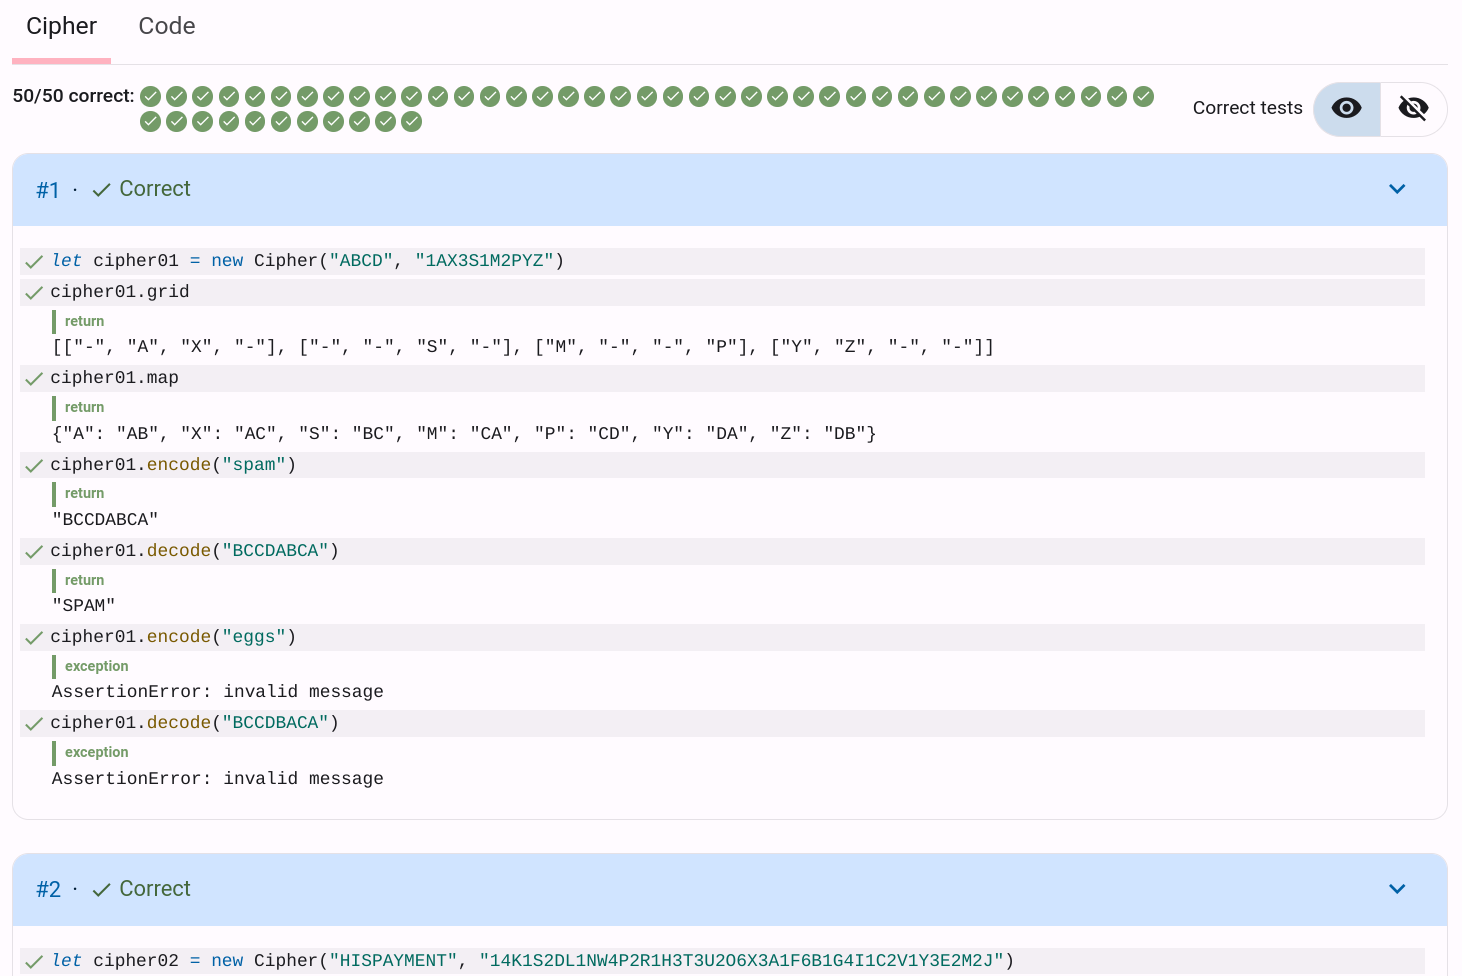
\includegraphics[width=\textwidth]{render-cipher}
    \caption{Dodona rendering of test results after TESTed validated a correct JavaScript submission for the programming exercise configured with the language-agnostic test suite from \vref{lst:cipher-example}. All tests from a single test case are visually grouped inside a card. Green check marks show that all tests of each script succeeded. Each expression has one reported output -- either its return value (\texttt{return}) or a runtime exception (\texttt{exception}) -- that is validated to be correct as indicated by the green color of the header for the reported output.\label{fig:dodona-render-cipher}}
\end{figure}

Parallel to dynamic testing, TESTed flags programming errors, bugs, stylistic errors and suspicious constructs by running a language-specific linter (see \vref{subsec:static-analysis-of-the-submission}) on each submission~\autocite{truongLearningProgramWeb2005}.
Dodona displays these linter messages inline in the source code of the submission, in a separate tab called Code.
Linters are preconfigured in the language-specific modules of TESTed, so no additional configuration is needed in the test suite.
Test suites may, however, overrule these linter configurations.

\subsubsection{Recoupling exercise: multiple functions and advanced data types}\label{subsubsec:recoupling-exercise:-multiple-functions-and-advanced-data-types}

\Vref{lst:recouple-example} shows a language-agnostic test suite for an exercise\footnote{\url{https://dodona.be/en/activities/1145516160/}} that asks to implement two functions: \texttt{divide} and \texttt{recouple}.
The first function must divide the given string into a number of parts.
The second function must split each given string and then recombine the corresponding parts into new strings.
As part of the problem-solving process, students may discover a divide-and-conquer strategy: the implementation of the second function may call the first function that solves a subtask.
However, the test suite validates the correct behavior of both functions in two separate units.
This example illustrates that TESTed-DSL allows leaving out the grouping of tests in a script as a shorthand for the common case of test cases whose script has a single test.
The first two test cases for the \texttt{divide} function (lines 4--7) use the \texttt{return} attribute with flow style notation of a YAML sequence to specify the function call is expected to return a sequence of strings as basic types of TESTed.
As a result, both lists and tuples will, for example, be accepted for Python submissions.
On the contrary, the first two test cases for the \texttt{recouple} function (lines 11--14) use an explicit cast to force the return value to be a list (line 12) or a tuple (line 14) for languages like Python that make the difference.
For Java and JavaScript submissions, however, arrays are accepted in both cases.
The same observation holds for the first argument passed to the function: a list (line 11) or a tuple (line 13) for languages that make the difference, or the default sequence type for other languages.

\begin{listing}
    \begin{minted}{yaml}
units:
  - unit: "Divide"
    scripts:
      - expression: "divide('accost', 3)"
        return: ["ac", "co", "st"]
      - expression: "divide('COMMUNED', 4)"
        return: ["CO", "MM", "UN", "ED"]
      - expression: "divide('programming', 5)"
        exception: "invalid division"
  - unit: "Recouple"
    scripts:
       - expression: "recouple(['ACcoST', 'COmmIT', 'LAunCH', 'DEedED'], 3)"
         return: !list ["ACCOLADE", "communed", "STITCHED"]
       - expression: "recouple(('ACCOLADE', 'communed', 'STITCHED'), 4)"
         return: !tuple ["ACcoST", "COmmIT", "LAunCH", "DEedED"]
       - expression: "recouple(['programming', 'computer', 'games'], 5)"
         exception: "invalid division"
    \end{minted}
    \caption[]{
        Language-agnostic test suite to validate correct behavior of submissions that must define the functions \texttt{divide} and \texttt{recouple}.
        Because each test case has a single test, grouping of tests in a script can be left out from the test suite specification as a shorthand.
    }
    \label{lst:recouple-example}
\end{listing}

Separating validation of the two functions across two separate units allows students to pinpoint immediately from the feedback what functions already behave as expected.
\Vref{fig:dodona-render-recouple} shows a Dodona rendering of the generated feedback for a Python submission whose implementation of the first function passes all tests.
However, the second function has three tests that fail for different reasons.
The first function call returns the correct result, but also writes the string \texttt{spam} to standard output (\texttt{stdout}) whereas no output is expected on this output stream.
The second function call returns a list where a tuple was expected.
The third function call should throw an exception, but this does not happen.

\begin{figure}
    \centering
    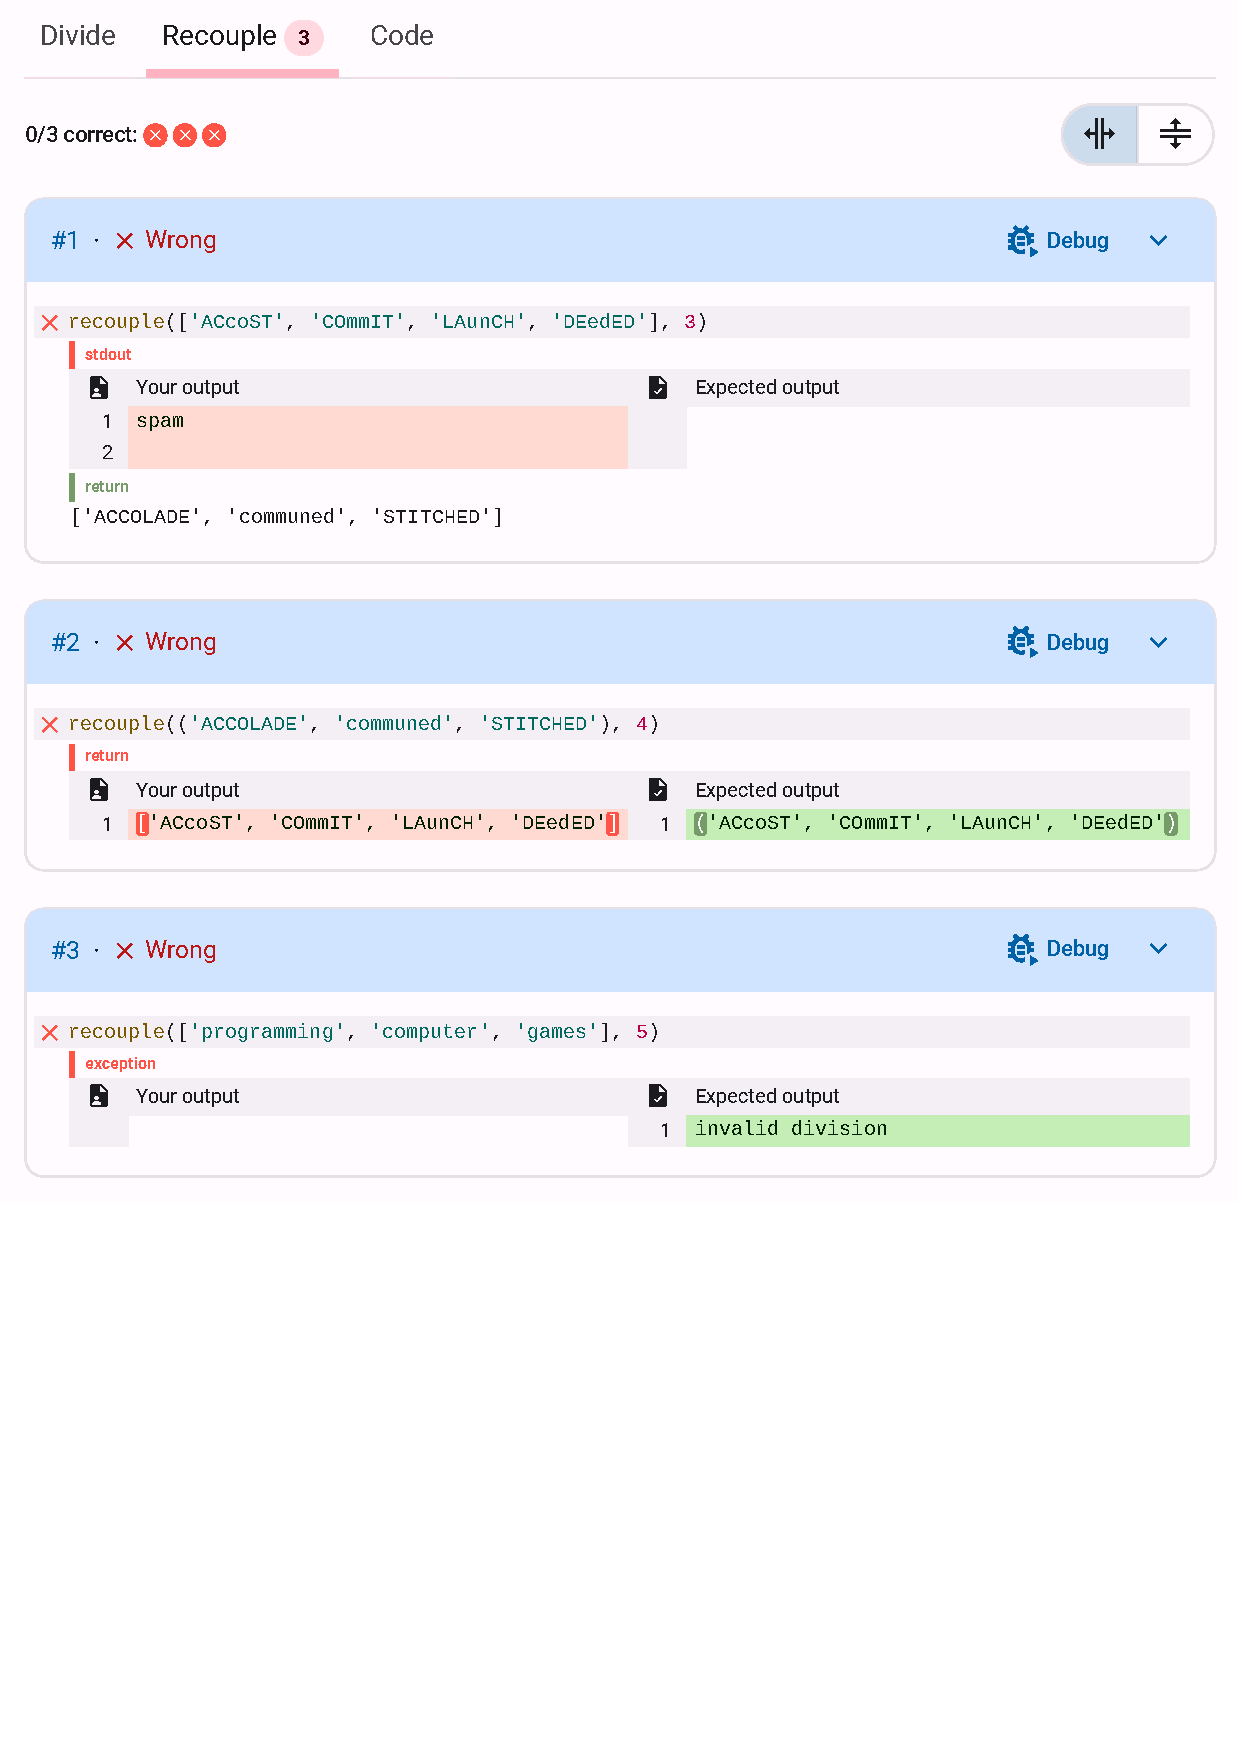
\includegraphics[width=\textwidth]{render-recouple}
    \caption{Dodona rendering of test results after TESTed validated a wrong Python submission for a programming exercise configured with the language-agnostic test suite from \vref{lst:recouple-example}. All test cases succeed for the implementation of the function \texttt{divide}, but for different reasons, some test cases fail for the implementation of the function \texttt{recouple}. An extra badge in the tab header displays the number of failing test cases in the corresponding unit, or the number of source code annotations in case of the Code tab (none in this case).\label{fig:dodona-render-recouple}}
\end{figure}

\subsubsection{Sum of three cubes exercise: I/O-stream testing and custom oracles}\label{subsubsec:sum-of-three-cubes-exercise:-i/o-stream-testing-and-custom-oracles}

Listing~\ref{lst:sum-example} shows a test suite for an I/O-stream based exercise that asks to read an integer $k$ from standard input and write a solution of the sum of three cubes problem ($x^3 + y^3 + z^3 = k$) to standard output as three lines containing non-zero integers $x$, $y$ and $z$~\autocite{bookerCrackingProblem332019}.
The test suite has one unit with three test cases whose script only specifies a single line of input streamed into standard input of the main call and three expected lines of output printed on standard output.
So again the shorthand structure applies here for units and scripts.
The first two test cases show different YAML alternatives for specifying multiline strings (line 4 and lines 6--9) as the expected value streamed to standard output.
However, specifying a fixed expected output is problematic for this exercise.
The task description does not imply any order in which the three integers must be listed, so any permutation of the three integers given by the expected solution for the second test case should also be validated as a correct solution.
Moreover, some values of $k$ have alternative solutions, irrespective of permutations.
For example, another way to solve the first test case is given by $(-5)^3 + 4^3 + 4^3 = 3$~\autocite{sutherlandSumsThreeCubes2019}.
As enumerating all possible solutions (and their permutations) is infeasible, the specification of the third test case provides a better approach.
TESTed uses the function \texttt{sum\_of\_three\_cubes} from the Python module \texttt{oracle.py} as a custom oracle to validate the correctness of the output generated on stdout.
TESTed always passes the actual output and some metadata, such as the programming language, and the expected output as the first argument to the oracle.
Additionally, extra arguments taken from the test suite can be passed (in this case there is only one extra argument: the integer \texttt{42}).

\begin{listing}
    \begin{minted}{yaml}
- unit: "Sum of three cubes"
  scripts:
    - stdin: "3"
      stdout: "1\n1\n1\n"
    - stdin: "33"
      stdout: |
        8866128975287528
        -8778405442862239
        -2736111468807040
    - stdin: "42"
      stdout:
        data: |
          -80538738812075974
           80435758145817515
           12602123297335631
         oracle: custom_check
         name: "sum_of_three_cubes"
         file: "oracle.py"
         arguments: [42]
    \end{minted}
    \caption[]{
        Language-agnostic test suite to validate correct behavior of submissions for an I/O-stream based exercise that asks to read an integer \(k\) from standard input and write a solution of the sum of three cubes problem \((x^3 + y^3 + z^3 = k)\) to standard output as three lines containing non-zero integers \(x\), \(y\) and \(z\).
    }
    \label{lst:sum-example}
\end{listing}

\begin{enumerate*}[label=\emph{\roman*})]
    \item share the same declarative structure and testing functionality across programming languages,
    \item bridge the gap between I/O-stream testing and unit testing, and
    \item allow for expressing test code in a language-agnostic way.
\end{enumerate*}

The custom oracle needs to
\begin{enumerate*}[label=\emph{\roman*})]
    \item check the output string has the correct format (three lines containing one integer each),
    \item parse the three integers $x$, $y$ and $z$ from the output (converting their string representation into integers) and
    \item check the integer expression $x^3 + y^3 + z^3$ yields the value of the second argument (\texttt{42}).
\end{enumerate*}
Passing an extra argument is not strictly needed here as the custom oracle could also derive the data from the expected value, using the same procedure as used to derive the data from the actual value.

\subsection{Language-agnostic task descriptions}\label{subsec:example-language-agnostic-task-descriptions}

\Vref{lst:task-description-markdown} shows a language-agnostic task description for the ``Recoupling'' exercise that was introduced in \vref{subsubsec:recoupling-exercise:-multiple-functions-and-advanced-data-types}.
The task description is specified using Kramdown-flavored Markdown.
It contains Jinja2 placeholders (\mintinline{jinja}{{{code}}}) for function names and formal/informal names of data types, along with MathJax placeholders (\mintinline{jinja}{$$...$$}) for \LaTeX{} formulas.
The task description ends with some examples of the expected behavior when calling the two functions \texttt{divide} and \texttt{recouple} that must be implemented for this programming exercise.
The language-agnostic specification of the sample code is denoted using the same specification of the test suite for the programming exercise in TESTed-DSL format or a reduced version thereof (see \vref{lst:recouple-example}).

\begin{listing}
    \begin{minted}[fontsize=\footnotesize]{jinja}
Write a function `{{function('divide')}}` that takes two arguments: _i_) a word (`{{datatype('text')}}`) and _ii_) the number of (non-overlapping) groups $$n \in \mathbb{N}_0$$ (`{{datatype('integer')}}`) into which the word must be divided. If the word passed to the function `{{function('divide')}}` cannot be divided into $$n$$ groups that have the same length, an exception must be raised with the message `invalid division`. Otherwise, the function must return a {{datatype('list').singular}} (`{{datatype('list')}}`) containing the $$n$$ groups (`{{datatype('text')}}`) into which the given word can be divided. All groups need to have the same length (same number of letters).

Write another function `{{function('recouple')}}` that takes two arguments: _i_) a {{datatype('sequence').singular}} (`{{datatype('sequence')}}`) of $$m \in \mathbb{N}_0$$ words (`{{datatype('text')}}`) and _ii_) the number of (non-overlapping) groups $$n \in \mathbb{N}_0$$ (`{{datatype('integer')}}`) into which the words must be divided. If at least one of the words passed to the function `{{function('recouple')}}` cannot be divided into $$n$$ groups that have the same length, an exception must be raised with the message `invalid division`. Otherwise, the function must return a {{datatype('sequence').singular}} containing the $$n$$ new words (`{{datatype('text')}}`) obtained when each of the $$m$$ given words is divided into $$n$$ groups that have the same length, and if each of the $$m$$ corresponding groups is merged into a new word. The type of the returned {{datatype('sequence').singular}} (`{{datatype('sequence')}}`) must correspond to the type of the {{datatype('sequence').singular}} passed as a first argument to the function.

### Example

```dsl

```
    \end{minted}
    \caption[]{
        Language-agnostic task description for the ``Recoupling'' exercise.
        The Kramdown-flavored Markdown contains Jinja2 placeholders for function names and both formal and informal names of data types.
        The task description ends with some examples that illustrate how the two functions should be used.
        The sample code is denoted using the same specification of the test suite for the programming exercise in TESTed-DSL format (\vref{lst:recouple-example}).
    }
    \label{lst:task-description-markdown}
\end{listing}

For the sample code in the template, we use the Jinja2 import facilities to include the test suite from \vref{lst:recouple-example}.
TESTed will automatically generate an example based on this test suite, while ignoring structural elements (like the hierarchy).

Starting from a task description template, the TESTed template engine can generate language-specific versions of the task description for all supported programming languages (\vref{fig:dodona-render-task-description}).
This is done by taking into account language-specific conventions (naming, quoting, formal and informal names and syntax for literals, expressions, and statements) as specified in the language modules for the supported programming languages.
This dual use between test suites and task description keeps the language-specific modules of TESTed lightweight and guarantees consistency between the generation of language-specific tests and descriptions.

\begin{figure}
    \centering
    \begin{tikzpicture}
        \node[anchor=south west,inner sep=0] (image1) at (0,0) {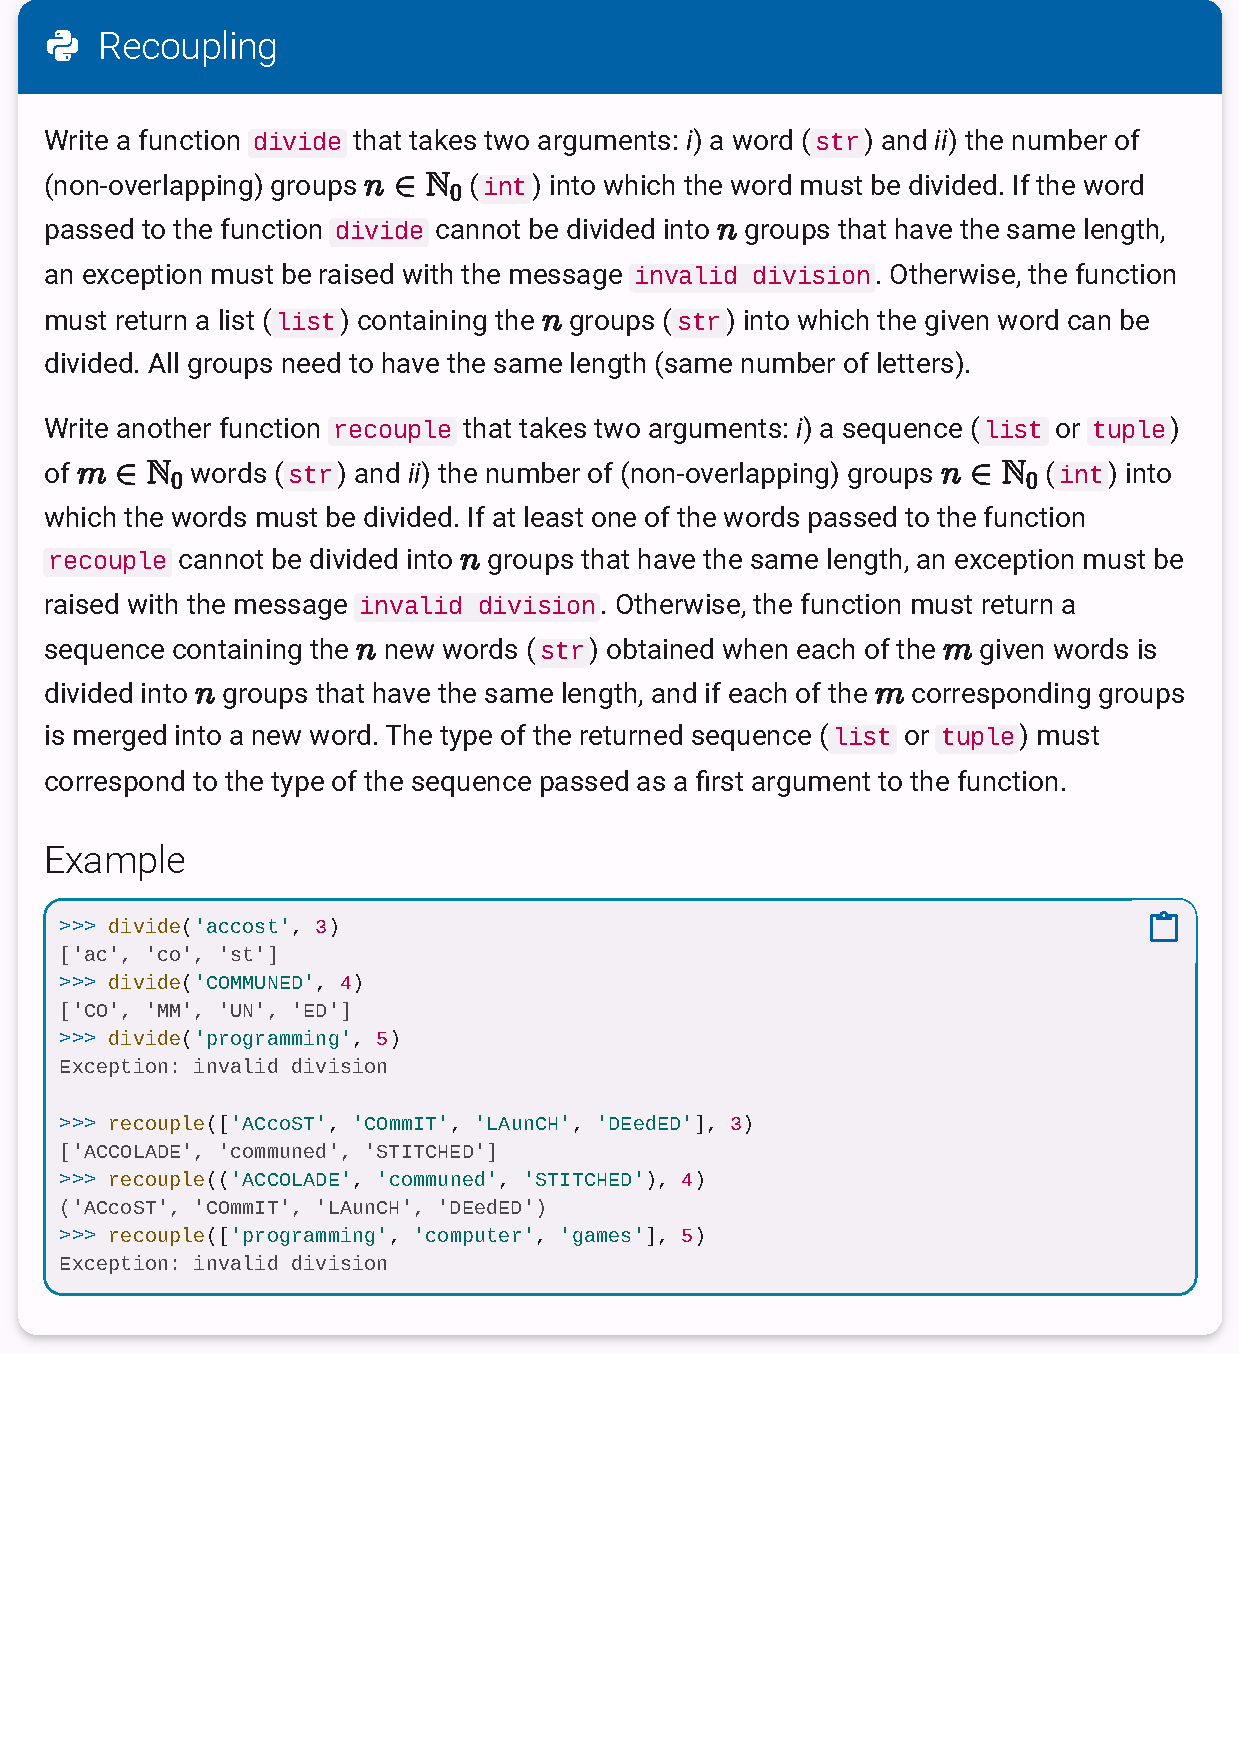
\includegraphics[width=0.65\textwidth]{recoupling-py}};
        \node[anchor=south west,inner sep=0] (image2) at (0.35\textwidth,-5) {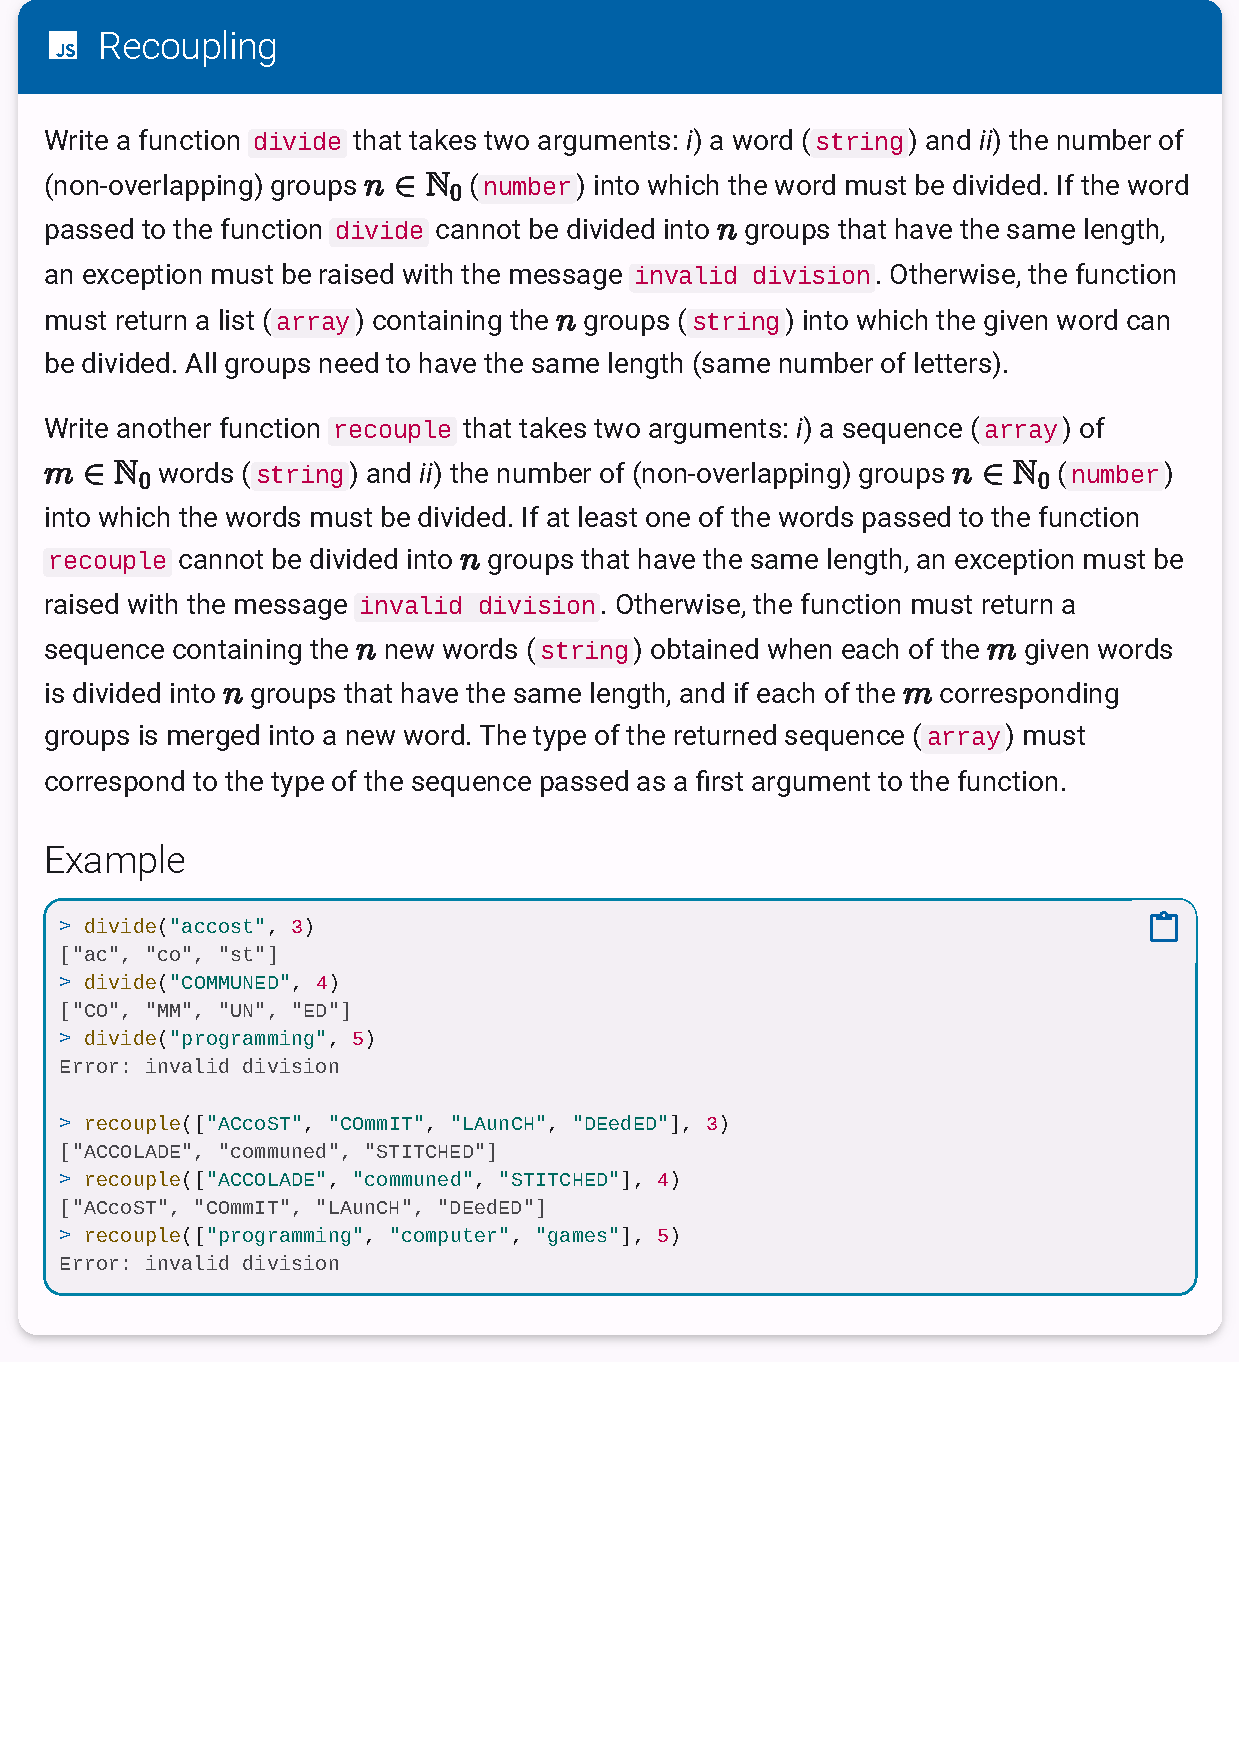
\includegraphics[width=0.65\textwidth]{recoupling-js}};
    \end{tikzpicture}
    \caption{Dodona rendering the Python (top left) and JavaScript (bottom right) versions of the task description as generated by the template engine of TESTed.\label{fig:dodona-render-task-description}}
\end{figure}

\section{Evaluation}\label{sec:dsl-evaluation}

During the academic year 2023--2024 we started promoting TESTed with its DSL as the primary way to author new (language-agnostic) programming exercises on Dodona~\autocite{vanpetegemDodonaLearnCode2023}.
We clearly documented the process, including guides and reference documentation.\footnote{\url{https://docs.dodona.be/nl/guides/exercises/} (some documentation is currently only available in Dutch).}
At the time of writing, \num{1124} programming exercises on Dodona support automated assessment through TESTed, with \num{333195} assessed student submissions (\vref{tab:exercises-on-dodona}).

\begin{table}
    \centering%
    \caption{Dodona programming exercises using TESTed for automated assessment.\label{tab:exercises-on-dodona}}%
    \addfontfeature{Numbers={Lining, Monospaced}}
    \small%
    \begin{tabular}{|l|r|r|}
        \hline
        \textbf{Programming language}   & \textbf{№ of exercises}   & \textbf{№ of submissions} \\
        \hline
        Bash                            & \num{32}                  & \num{121011}              \\
        C                               & \num{83}                  & \num{652}                 \\
        C\#                             & \num{1}                   & \num{6}                   \\
        Haskell                         & \num{86}                  & \num{241}                 \\
        Java                            & \num{120}                 & \num{1493}                \\
        JavaScript                      & \num{271}                 & \num{178011}              \\
        Kotlin                          & \num{146}                 & \num{271}                 \\
        Python                          & \num{385}                 & \num{31510}               \\
        \hline
        \textbf{Total}                  & \textbf{\num{1124}}       & \textbf{\num{333195}}     \\
        \hline
    \end{tabular}
\end{table}

In the next sections, we look into a case study where we converted all JavaScript exercises of a course to use TESTed and its DSL\@.
This resulted in \num{72} programming exercises and \num{22018} student submissions (these are part of the total numbers shown in \vref{tab:exercises-on-dodona}).

\subsection{Expressiveness and ergonomics}\label{subsec:dsl-expressiveness-and-ergonomics}

To evaluate the expressiveness of TESTed-DSL and its applicability in educational practice, we authored test suites for a collection of \num{72} programming exercises that were used during the 2023 spring semester in a CS1 course at Ghent University, Belgium taken by \num{114} students.\footnote{\url{https://dodona.be/en/courses/2263/}}
None of these exercises is I/O-stream based, \num{22} ask to implement one or more functions and \num{50} ask to implement one or more classes.

The largest part of the collection consists of all the \num{66} JavaScript exercises we designed for this course over the years.
These exercises already supported automated assessment with a test suite designed for a custom JavaScript-specific testing framework.
To migrate automated assessment for these exercises to TESTed, we wrote a script that either converts their existing JavaScript test suites into a TESTed-DSL specification or reports why this is not possible.
Seamless automated conversion was helped by the fact that we designed TESTed according to best practices we obtained from designing and implementing many language-specific testing frameworks for Dodona, and a generic feedback format (JSON) that closely follows the structure of TESTed-DSL test suites.

All existing test suites for these JavaScript exercises could be transformed into TESTed-DSL: \num{58} of \num{66} (\qty{88}{\percent}) into language-agnostic test suites and \num{8} of \num{66} (\qty{12}{\percent}) into JavaScript-specific test suites.
The latter use JavaScript-specific language constructs that are not (yet) supported by TESTed: array indexing, object indexing, array destructuring assignment, object identity checking (\mintinline{javascript}{===} operator), class constants, spread syntax (\mintinline{javascript}{...} operator), and the use of arrow functions as callbacks.
The sample solutions for the programming exercises -- assumed to be correct -- were used for testing the test suite migration throughout the process.

Although the above experiment made clear that most, but not all, test suites for existing JavaScript exercises could be converted into language-agnostic test suites for TESTed, TESTed-DSL was expressive enough to also specify JavaScript-specific test suites for the remaining exercises.
At least we may conclude from this experiment that for our practice, we can gradually deprecate language-specific testing frameworks in favor of TESTed.
Along the way, converting test suites into a language-agnostic TESTed-DSL specification also broadens the usability of the programming exercises across programming languages.

We also added 6 new programming exercises with language-agnostic TESTed-DSL test suites to the collection, designed from scratch and used for a midterm test (2 exercises) and for 2 exam sessions (2 exercises each) during the semester.
Our experience in doing so is that direct authoring of TESTed-DSL test suites is very ergonomic, either when done by hand or using a generator script based on a correct solution.
Human error is reduced by using the formal specification for automatic verification that TESTed-DSL test suites are well-formed and valid.
TESTed performs such verification while parsing test suites, but this can also be done interactively while authoring the test suites in an \textsc{ide}.
For example, we provide a VS Code Plugin\footnote{\url{https://marketplace.visualstudio.com/items?itemName=dodona.dodona-exercise-plugin}} that automatically applies the JSON Schema of the DSL to catch errors and to provide autocompletion.
The improved readability of TESTed-DSL test suites further increases productivity and enhances comfort while authoring programming exercises, especially with \textsc{IDE}-support for syntax highlighting and autocompletion.

Of these exercises, \num{19} were used as mandatory assignments during the 2023 spring semester of the CS1 course and \num{6} for midterm tests and exams.
Students could use the remaining exercises from the collection for additional practice in preparation for tests and exams.
Students were not restricted in the number of submissions for each exercise.
They received immediate feedback from automated assessment upon each submission, also after the submission deadline and also during midterm tests and exams.
Students had previous experience in working with Dodona for solving Java, Python and Bash programming exercises with automated assessment.
But most of them had no prior experience with the collection of JavaScript exercises, nor with automated assessment based on the custom JavaScript-specific testing framework used in previous editions of the course.
For each course edition, we make a different selection of mandatory exercises and we always design new exercises for midterm tests and exams.
This way, students who had to retake the course had no reference for comparison between the custom JavaScript-specific testing framework used in previous course editions and TESTed using during the 2023 edition.
For that reason, we decided not to inform students about us switching the JavaScript testing framework that for them runs as a hidden component in the backend of Dodona.

In total, TESTed automatically assessed \num{22018} JavaScript submissions during the 2023 spring semester of the course.
None of the questions we received from students during the hands-on sessions for the course or via Dodona's Q\&A module hinted at any issues with automated assessment or the feedback it generated other than content-related issues.
We also found no indications of problems in the course evaluation that students complete some weeks after the end-of-semester exams.

\subsection{Performance}\label{subsec:dsl-performance}

As is the case for software testing in general, the user experience of educational software testing depends on the performance of test runs to limit how long students must wait before feedback is reported~\autocite{sarsaSpeedingAutomatedAssessment2022}.
We therefore ran a benchmark using all 72 JavaScript exercises mentioned previously to validate the performance of TESTed.
These exercises have 95 test cases on average, with a minimum of 2 and a maximum of 518.
Previously, we showed that the extra flexibility provided by language-agnostic testing comes with an acceptable overhead when dynamically generating test code for language-specific test harnesses (\vref{subsec:tested-in-educational-practice}).
Here, we specifically investigated if using a DSL for specifying test suites incurs additional overhead compared to using the JSON-formatted test suite specifications introduced in version 1.0 of TESTed.
The latter specifications closely reflect the internal structure and functionality of the testing framework, whereas TESTed-DSL was designed to make test suite authoring as ergonomic as possible.

The benchmark was run on a laptop running Linux (NixOS version 24.05) with \qty{32}{\gibi\byte} \textsc{ram}, an Intel i7-11850H processor, and a \qty{1}{\tebi\byte} \textsc{ssd}.
No power-saving features were active during the benchmark.
It turns out that parsing and processing of TESTed-DSL test suites take \qty{20}{\percent} less time on average compared to the original \textsc{json}-formatted test suites.
We believe this is mainly due to using a more performant YAML parsing library compared to the Python built-in JSON parsing library.
However, this illustrates TESTed-DSL does not incur any additional overhead compared to the original JSON format.
Because the DSL still supports all features of TESTed, we decided to deprecate support for JSON-formatted test suites in favor of TESTed-DSL\@.

Equally important is the total runtime for assessing the submissions for a programming exercise.
This is the time students must wait before feedback is available.
We observed that \qty{75}{\percent} of all JavaScript exercises are assessed automatically in less than 725 ms (\vref{fig:dsl-performance}).
On average, TESTed spends \qty{225}{\milli\second} parsing and processing a TESTed-DSL test suite, with the remaining time used for generating test code (language-specific test harnesses), running test code and checking test results.
Due to additional speedups in the testing framework itself, TESTed 2.0 is up to 2.8 times\footnote{\url{https://github.com/dodona-edu/universal-judge/pull/334}} faster than TESTed 1.0 (both using JSON test suites).

\begin{figure}
    \centering
    \includestandalone{performance}
    \caption{Histogram and box plot of the total runtime for automatically assessing the (correct) sample solutions with TESTed for all \num{72} JavaScript exercises.
    Half of the programming exercises have their submissions assessed in the range of \SIrange{360}{725}{\milli\second}, with \qty{75}{\percent} of the assessments taking less than \qty{725}{\milli\second}.\label{fig:dsl-performance}}
\end{figure}

\section{Results and contributions}\label{sec:dsl-results-and-contributions}

In this section, we discuss TESTed-DSL and its impact on authoring test suites and task descriptions for programming exercises that support automated assessment.
Apart from its application in authoring language-agnostic task descriptions, the three main contributions of TESTed-DSL for authoring test suites are in expressing how the requirements of programming exercises must be assessed.
Its test suites:

\begin{enumerate}
    \item share the exact same declarative structure and functionality across programming languages,
    \item bridge between I/O-stream testing (black-box, weakly typed) and unit testing (white-box, strongly typed), and
    \item can express the test code in a language-agnostic way.
\end{enumerate}

The first contribution might be of general interest to the broader software engineering community, but the last two contributions are especially relevant for computer science education.
In the following subsections, we discuss the impact of each contribution.

For task descriptions, many of the same benefits apply as for test suites.
Specifically, the application of the DSL to task descriptions allows for programming language agnostic representations of code references: names of constructs (functions, classes, properties, etc.) and data types (e.g.\ lists, sets).
Additionally, code fragments written in the abstract language can be automatically converted to code fragments of the target programming language.

\subsection{Declarative structure}\label{subsec:dsl-declarative-structure}

Most programming languages have one or more unit testing frameworks, whose structure and functionality are predominantly derived from Smalltalk's SUnit~\autocite{beckSimpleSmalltalkTesting1997}.
Collectively the latter are known as xUnit~\autocite{meszarosXUnitTestPatterns2007}.
xUnit frameworks are code-driven as their test suites express both the structure and the behavior of tests in the same programming language as the software under test.
Strong coupling to the language of the software under test is natural as behavioral tests must access its public interfaces.
In contrast, TESTed-DSL separates these two concerns by expressing the structure of test suites in a declarative way (in YAML).
TESTed implements the functionality for processing this structural part of test suites in its core module, so only a single highly-optimized implementation is needed for this shared functionality of unit testing across programming languages.
Functionality that remains language-dependent is the generation of test harnesses.
But TESTed splits that across its core module generating language-agnostic harnesses and language-specific modules generating language-specific harnesses, to keep the language-specific modules as lightweight as possible and to share common functionality.

TESTed allows to specify language-specific test suites expressed in TESTed-DSL that share the same structure across programming languages.
TESTed simply has to copy the language-specific attributes when generating language-specific test harnesses.
As an example, \vref{lst:javascript-test-suite} shows a JavaScript-specific version of the test suite from \vref{lst:cipher-example}.
Test suites guiding automated assessment for the same exercise in other programming languages supported by TESTed, only differ in their representation for statements of the test scripts (\texttt{expression}, \texttt{statement}), expected values for strongly typed outputs (\texttt{return}, \texttt{exception}) and strongly typed arguments passed to custom oracles (\texttt{arguments}).
The programming language in which these attributes (blue background) are expressed is specified with the \texttt{language} attribute (line 2) that is inherited across the hierarchy of the test suite.

\begin{listing}
    \begin{minted}[escapeinside=@@]{yaml}
unit: "Cipher"
language: @\hl{"javascript"}@
cases:
  - script:
      - statement: @\hl{"const cipher = new Cipher('ABCD', '1AX3S1M2PYZ')"}@
      - expression: @\hl{"cipher.grid"}@
        return:
         - ["-", "A", "X", "-"]
         - ["-", "-", "S", "-"]
         - ["M", "-", "-", "P"]
         - ["Y", "Z", "-", "-"]
      - expression: @\hl{"cipher.map"}@
        return:
          "Y": "DA"
          "M": "CA"
          "P": "CD"
          "Z": "DB"
          "S": "BC"
          "A": "AB"
          "X": "AC"
      - expression: @\hl{"cipher.encode('spam')"}@
        return: "BCCDABCA"
      - expression: @\hl{"cipher.decode('BCCDABCA')"}@
        return: "SPAM"
      - expression: @\hl{"cipher.encode('eggs')"}@
        exception: "invalid message"
      - expression: @\hl{"cipher.decode('BCCDBACA')"}@
        exception: "invalid message"
  - script:
      # statements and expressions of the second script come here
    \end{minted}
    \caption[]{
        JavaScript-specific test suite to validate correct behavior of submissions that must define the class \texttt{Cipher}, where the shorthand was applied for test suites having a single unit.
        The JavaScript-specific attributes of this test suite are highlighted in blue.
    }
    \label{lst:javascript-test-suite}
\end{listing}

A single TESTed-DSL test suite can also specify language-specific alternatives for multiple languages, as opposed to using a separate unit testing framework for each language, each with their custom version of the test suite.
\Vref{lst:multiple-test-suite} shows an example with Python and JavaScript alternatives for the same test expression.
This gives access to language-specific features that are not (yet) supported in the abstract programming language of TESTed-DSL or are not (yet) supported by a language-specific module of TESTed.
Here, the former is the case for passing anonymous functions as arguments to functions and converting strings to uppercase.
This example also shows that TESTed-DSL test suites can mix language-specific (lines 2-4) and language-agnostic (line 5) sections.

% TODO: text colors...
\begin{listing}
    \begin{minted}[escapeinside=@@]{yaml}
unit: 'Sort words'
expression:                       # language-specific
  python: @\hl[ugent-ps!20!white]{"sort\_words(['SPAM', 'eggs', 'bacon'], lambda word: word.upper())"}@
  javascript: @\hl{'sortWords(["SPAM", "eggs", "bacon"], word => word.toUpperCase())'}@
return: ['bacon', 'eggs', 'SPAM'] # language-agnostic
    \end{minted}
    \caption[]{
        TESTed-DSL test suite to validate correct behavior of submissions that must either define the function \texttt{sort\_words} in Python or define the function \texttt{sortWords} in JavaScript. The Python-specific sections of this test suite are marked in green and the JavaScript-specific sections in blue.
    }
    \label{lst:multiple-test-suite}
\end{listing}

\subsection{Combined I/O-stream and unit testing}\label{subsec:combined-i/o-stream-and-unit-testing}

The examples in \vref{sec:dsl-illustrative-examples} already show the flexibility of TESTed-DSL to specify test suites for both I/O-stream based exercises (\vref{lst:sum-example}) and exercises with fixed internal interfaces (\vref{lst:cipher-example,lst:recouple-example}).
However, individual tests can also combine any mix of weakly and strongly typed input and output channels.
For example, an expression calling a function with arguments, which reads from stdin, accesses main call arguments and environment variables, writes to stdout and stderr and returns a value.
In addition, test cases can combine black-box tests for the main call with a test script of white-box tests for statements and expressions that can access internal interfaces of the submission.
This unification of test suites combining strongly/weakly typed and black-box/white-box approaches solves a long-standing problem in educational software testing.

\Citeauthor{fonteFlexibleDynamicSystem2013} proposed Output Semantic-Similarity Language (\textsc{ossl}) ~\autocite{fonteFlexibleDynamicSystem2013} as a domain-specific language to serialize strongly typed data across weakly typed I/O-streams.
Although the formal specification of \textsc{ossl} resembles the TESTed basic types supported by TESTed-DSL, no OSSL-parser was ever published and it was only conceived for use in language-agnostic I/O-stream testing.
For application in language-specific unit testing, TESTed added the extra layer of advanced types that are also supported by TESTed-DSL\@.
\Citeauthor{enstromFiveYearsKattis2011} suggest splitting programming exercises with complex tasks over multiple exercises, each testing a separate subtasks via I/O-stream testing~\autocite{enstromFiveYearsKattis2011}.
Compared to the approach taken by TESTed-DSL, this feels like a poor man's version of white-box testing.
It forces students to reveal internal interfaces via standard I/O-streams and at the same time asks authors to design and maintain alternative instances of an exercise.
An accumulation of extra work, where what we actually seek are ways to reduce the work of authoring and solving programming exercises~\autocite{douceAutomaticTestbasedAssessment2005}.

\textsc{acm/icpc} programming contests and derivatives are another area where I/O-stream based programming exercises are regularly used.
These exercises often follow a specific style, with multiple test cases bundled in a single input stream.
This style dates back from times where judges -- as automated software testing frameworks are commonly called in the context of programming contests -- were restricted to a single execution of the submission's main function.
These platforms are heavily used in classrooms~\autocite{wasikSurveyOnlineJudge2018,zinovievaUseOnlineCoding2021}.

Although the \textsc{acm/icpc} style of testing can be expressed using TESTed-DSL test suites, it forces students to implement a main function that loops over test cases and bundles their output in a single output stream.
This approach of packing multiple test cases into a single test case further increases the black-box nature of testing.
Additionally, it may propagate faults in the implementation of submissions as a failure for one test case to failures for successive test cases, making it harder to report feedback that easily discerns which individual test cases pass or fail.
In programming contests, limiting feedback to reporting whether all test cases passed is not a concern.

However, in an educational context, we do strive for rich and fine-grained feedback, meaning an automated testing framework designed for contests is less ideal.
In TESTed-DSL, we essentially move the responsibility for processing multiple test cases from the student to the test framework.
This is useful for all students, but especially benefits those students with limited programming experience.

\subsection{Language-agnostic testing}\label{subsec:language-agnostic-testing}

TESTed-DSL's declarative structure to organize multiple test cases and describe individual test cases already enables authoring programming exercises whose submissions can be automatically assessed across programming languages.
The abstract programming language means that test statements and strongly typed expected outputs can be specified once for all supported programming languages, eliminating repetition for each individual language that is a target for the programming exercise.

The need for language-agnostic software testing is relatively unique to programming exercises, where it is also highly relevant to support automated assessment.
Beyond this educational context, we do not see many use cases for having a single specification to test multiple implementations that differ in programming language.
Those use cases do exist (e.g.\ testing multiple implementations of the same standard), but they are often limited to I/O-stream testing.

Besides online learning platforms supporting computer sciences courses in secondary and higher education, some platforms target self-learning, programming contests or recruitment~\autocite{hidalgo-cespedesEvaluationOnlineJudge2023}.
Examples include CodeWars\footnote{\url{https://www.codewars.com/}}, Edabit\footnote{\url{https://edabit.com/}}, LeetCode\footnote{\url{https://leetcode.com/}}, CheckIO\footnote{\url{https://checkio.org/}}, Exercism\footnote{\url{https://exercism.org/}} and CodingBat\footnote{\url{https://codingbat.com/}}.
As far as we know, TESTed is the only existing framework that bridges unit testing with language-agnostic testing.
Most other frameworks are either restricted to I/O-stream testing or rely on general-purpose unit testing frameworks.
The I/O-stream based approach forces students to implement an I/O-streaming model in the main function and test oracles to process weakly typed data, and can only evaluate the behavior of submissions as a whole.
Because general-purpose unit testing frameworks work with language-specific test suites, the alternative approach duplicates efforts in specifying the expected behavior for a programming exercise to each target programming language of its submissions.
This can be seen in how separate test suites are written for each target language in most programming platforms.
Only Exercism has a mechanism\footnote{\url{https://github.com/exercism/problem-specifications}} by which some exercises have a single specification in a generic track that is used to automatically derive language-specific instances.
This system shares its goals with TESTed-DSL\@.
However, it is far less flexible and ergonomic for authoring programming exercises, as the generation step is needed each time.

\section{Conclusions and future work}\label{sec:dsl-conclusion-and-future-work}

Version 2.0 of TESTed introduces TESTed-DSL as a domain-specific language for writing the test suites that underlie automated assessment, and for writing language-agnostic task descriptions.
We have paid special attention to performance to ensure that TESTed-DSL has no additional overhead compared to JSON test suites (in fact, TESTed-DSL is 1.2 times faster than JSON test suites).
TESTed-DSL itself, apart from its use in authoring language-agnostic task descriptions, has three main contributions: \begin{enumerate*}[label=\emph{\roman*})] \item sharing the same declarative structure across programming languages, \item bridging the gap between I/O-stream testing and unit testing, and \item allowing test code to be expressed in a language-agnostic way.\end{enumerate*}
The first contribution may be of general interest to the broader software engineering community, but the last two contributions are particularly relevant to computer science education.

Our goal is to further develop TESTed as an educational software testing framework for authoring different types of programming exercises across programming languages.
This paper has focused mainly on dynamic testing, but TESTed also performs compilation and linting as generic types of static testing that are preconfigured in the language-specific modules.
One area of future interest is the introduction of a language-agnostic API for static code analysis.

We are currently investigating possible extensions to the abstract language of TESTed-DSL, such as operators for testing operator overloading, string conversion, comments, indexing sequences, indexing mappings, destructuring, object identity checking, and object equivalence checking.
There is no need to conservatively restrict the abstract language to features supported by all or most programming languages, as TESTed automatically detects and reports features not supported by a specific programming language or not (yet) implemented by its language module.
Support for additional test inputs (file descriptors, environment variables) and outputs (file descriptors, global scope) is in progress.
We are also investigating native support for pretty printing of nested data structures to make it easier to detect differences between expected and actual return values, and data-driven tests (parameterized tests) to further improve the readability of test suites, support dynamic generation of test data and boost performance of running tests.
Our future roadmap also includes internationalization of named submission interfaces, different ways to measure code coverage, and support for hidden units/test cases that are visible to teachers but remain invisible to students to avoid gaming -- also known as programming to the test~\autocite{pevelerComparingJailedSandboxes2019}.

Further enhancements and improvements of TESTed will be driven by educational practice, with the creation of new programming exercises and the conversion of existing exercises to TESTed-DSL being a major driver.
Feel free to run TESTed as a standalone command line tool, integrate it into your online learning environments, and let us know about interesting use cases.
We ourselves now routinely rely on TESTed to create new programming exercises and to gradually migrate existing exercises to port them to other programming languages and to benefit from the additional features that TESTed brings.
We also switched to TESTed when training (secondary school) teachers how to create programming exercises with automated assessment for Dodona.
First of all because it covers most common cases, is easy to use, and teachers can use the same framework for educational software testing, regardless of their target programming language(s).
As an open-source project on GitHub\footnote{\url{https://github.com/dodona-edu/universal-judge}}, we welcome the sharing of unsupported exercise scenarios, bugs and feature requests documented as issues.
We also welcome additional language-specific modules to support new programming languages\footnote{\url{https://docs.dodona.be/en/references/tested/new-programming-language/}}.

\end{document}
